\documentclass[twoside]{amsart}
\usepackage{amssymb,latexsym}
\usepackage{xspace}
\usepackage{enumerate}
\usepackage{graphics}
\newcommand{\Rationals}{\mathbb{Q}{}}
\newcommand{\Reals}{\mathbb{R}{}}
\newcommand{\Integers}{\mathbb{Z}{}}
\newcommand{\Solution}{\textsc{Solution}\xspace}
\newcommand{\Problem}{\textsc{Problem}\xspace}
\newcommand{\Blank}{\mathrel{\phantom{=}}}
\newcommand{\ltrue}{\top}
\newcommand{\lfalse}{\bot}
\begin{document}
\title{Answers to Chapter 4 Exercises - A Book of Abstract Algebra}
\author{Michael Welch}
\date{\today}
\maketitle

This document contains selected answers to exercises from chapter 4
of A Book of Abstract Algebra.

Remark on notation. In the exercises in this document, the exponential
notation $a^n$ is used in the following sense: if $a$ is any element of
a group $G$, then $a^2$ means $aa$, and $a^3$ means $aaa$, and, in
general, $a^n$ is the product of $n$ factors of $a$, for any positive
integer $n$.

\begin{enumerate}[A.]
   \item \textsc{Solving Equations in Groups}

   \noindent Let $a$, $b$, $c$, and $x$ be elements of a group $G$. In each of
   the following, solve for $x$ in terms of $a$, $b$, and $c$.

   \noindent   1. $axb = c$
      \begin{align*}
         axb & = c \\
	 a^{-1}axb & = a^{-1}c \\
	 xbb^{-1} & = a^{-1}cb^{-1} \\
	 x & = a^{-1}cb^{-1}
      \end{align*}

   \noindent   2. $x^2b = xa^{-1}c$
      \begin{align*}
         x^2b & = xa^{-1}c    \\
	 x^2bb^{-1} & = xa^{-1}cb^{-1} \\
	 x^2        & = xa^{-1}cb^{-1} \\
	 x^{-1}x^2  & = x^{-1}xa^{-1}cb^{-1}\\
	 x^{-1}xx   & = a^{-1}cb^{-1} \\
	 x          & = a^{-1}cb^{-1}
      \end{align*}

   Solve simultaneously:

   \noindent 3. $x^2a = bxc^{-1}$ and $acx = xac$
   \begin{align*}
      acx & = xac      & \text{Given} \\
      xacx & = x^2ac   & \text{Multiply by $x$} \\
      xacxc^{-1} & = x^2a \\
      xacxc^{-1} & = bxc^{-1} & \text{Substitute} \\
      xacx       & = bx  \\
      xac        & = b  \\
      x          & = bc^{-1}a^{-1}
   \end{align*}

   \noindent 4. $ax^2=b$ and $x^3=e$
   \begin{align*}
      ax^2 & = b     & \text{Given} \\
      ax^3 & = bx    & \text{Multiply, on right, by x} \\
      a    & = bx    & \text{Subst other given} \\
      x    & = ab^{-1}
   \end{align*}

   \noindent 5. $x^2 = a^2$ and $x^5 = e$
   \begin{align*}
      x^2 & = a^2   & \text{Given} \\
      x^2 x^2 & = a^2 x^2 & \text{Multiply on right by $x^2$}\\
      x^4     & = a^4     & \text{Because $x^2 = a^2$.}\\
      x^5     & = a^4x \\
      e       & = a^4x \\
      x       & = (a^4)^{-1}
   \end{align*}

   \noindent 6. $(xax)^3 = bx$ and $x^2 a = (xa)^{-1}$.
   \begin{align}
      (xax)^3  & = bx \\
      xaxxaxxax & = bx \\
      x^2a      & = (xa)^{-1} \\
      xxaxa     & = e  & \text{from 3} \\
      xaxxa     & = e  & \text{from 3} \\
      e xxax    & = bx & \text{subst 5 into 2} \\
      exxaxa    & = bxa & \text{mult by a on right} \\
      ee        & = bxa & \text{subst 4 into 7} \\
      b^{-1}    & = xa \\
      b^{-1}a^{-1} & = x  \\
      x & = (ab)^{-1}
   \end{align}

   \item \textsc{Rules of Algebra in Groups}
   For each of the following rules, either prove that it is true in 
   every group $G$, or give a counterexample to show that it is false in 
   some groups. (All the counterexamples you need may be found in the group
   of matrices $\{I,A,B,C,D,K\}$ described on page 28.)

   The matrices from page 28 and the matrix multiplication table
   are recreated in figure~\ref{tab:matrices} and table~\ref{tab:matmult}
   respectively.

   \begin{figure}
   \caption{The matrices of $G$.}
   \label{tab:matrices}
   \begin{align*}
     I & = \left( \begin{array}{rr} 
              1 & 0 \\ 
	      0 & 1
	   \end{array} \right) & 
     A & = \left( \begin{array}{rr}
              0 & 1 \\
	      1 & 0
	   \end{array} \right)  &
     B & = \left( \begin{array}{rr}
              0 & 1 \\
	      -1 & -1
	   \end{array}  \right) \\ \\
     C & = \left( \begin{array}{rr}
              -1 & -1 \\
	       0 &  1
	   \end{array} \right) &
     D & = \left( \begin{array}{rr}
              -1 & -1 \\
	       1 &  0
	   \end{array} \right) &
     K & = \left( \begin{array}{rr}
               1 &  0 \\
	      -1 & -1
	   \end{array} \right)
   \end{align*}
   \end{figure}

   \begin{table}
   \caption{Matrix multiplication of the matrices in $G$}
   \label{tab:matmult}
   \begin{tabular}{c|cccccc}
     $*$ & $I$ & $A$ & $B$ & $C$ & $D$ & $K$ \\ \hline
     $I$ & $I$ & $A$ & $B$ & $C$ & $D$ & $K$ \\
     $A$ & $A$ & $I$ & $C$ & $B$ & $K$ & $D$ \\
     $B$ & $B$ & $K$ & $D$ & $A$ & $I$ & $C$ \\
     $C$ & $C$ & $D$ & $K$ & $I$ & $A$ & $B$ \\
     $D$ & $D$ & $C$ & $I$ & $K$ & $B$ & $A$ \\
     $K$ & $K$ & $B$ & $A$ & $D$ & $C$ & $I$
   \end{tabular}
   \end{table}
   
   \noindent 1. If $x^2=e$, then $x=e$.

   \noindent \Solution This rule is false. A counter example is
   $A*A=I$ yet $A\ne I$.

   \noindent 2. If $x^2=a^2$ then $x=a$.

   \noindent \Solution This rule is false. A counter example is $A*A=I=I*I$
   yet $A \ne I$.

   \noindent 3. $(ab)^2 = a^2b^2$.

   \noindent \Solution This rule is false. A counter example is given
   by letting $a=A$ and $b=B$. $(AB)^2=C^2=I \ne D = ID = A^2B^2$.

   \noindent 4. If $x^2=x$, then $x=e$.

   \noindent \Solution This rule is true.
   \begin{proof}
      \begin{align*}
         x^2 & = x \\
	 xx  & = x \\
	 xxx^{-1} & = xx^{-1} \\
	 xe       &= e \\
	 x        & = e \qedhere
      \end{align*}
   \end{proof}

   \noindent 5. For every $x \in G$, there is some $y \in G$ such that
   $x = y^2$. (This is the same as saying that every element of $G$ has
   a ``square root''.)

   \noindent \Solution This rule is false. In the group G in
   figure~\ref{tab:matrices}, it is clear that the matrices 
   $A$, $C$, and $K$ do not have a ``square root''.

   \noindent 6. For any two elements $x$ and $y$ in $G$, there is an element
   $z$ in $G$ such that $y=xz$.

   \noindent \Solution. This rule is true.
   \begin{proof}
   We want to make the equality $y=xz$ hold. Since $G$ is a group we know
   that $x$ has an inverse. So we can write $z=x^{-1}y$. Also since
   $G$ is a group we know that $x^{-1}y$ is defined and unique. Therefore,
   $z$ exists.
   \end{proof}

   \item \textsc{Elements That Commute}

   \noindent If $a$ and $b$ are in $G$ and $ab=ba$, we say that $a$ and $b$ 
   \emph{commute}. Assuming that $a$ and $b$ commute, prove the following:

   \noindent 1. $a^{-1}$ and $b^{-1}$ commute.
   \begin{proof}
      \begin{align*}
         a^{-1}b^{-1} & = (ba)^{-1} && \text{Theorem 3} \\
	              & = (ab)^{-1} && \text{Given $a,b$ commute} \\
		      & = b^{-1}a^{-1} && \text{Theorem 3} \qedhere
      \end{align*}
   \end{proof}

   \noindent 2. $a$ and $b^{-1}$ commute. (\textsc{Hint}: First show
   that $a=b^{-1}ab$.
   \begin{proof}
   Since $ab=ba$, it is true that $ba=ab$ and $b^{-1}ba=b^{-1}ab$. This
   can be reduced and we have that $a=b^{-1}ab$. Finally, we can
   multiply by $b^{-1}$ on both sides to get $ab^{-1}=b^{-1}a$.
   \end{proof}

   \noindent 3. $a$ commutes with $ab$.
   \begin{proof}
   We know that $a(ab) = a(ba)$ by commutativity, and $a(ba)=(ab)a$ by
   associativity. So we have $a(ab)=(ab)a$.
   \end{proof}

   \noindent 4. $a^2$ commutes with $b^2$.
   \begin{proof}
      \begin{align*}
         a^2b^2 & = (aa)(bb) && \text{Definition}\\
	        & = a(a(bb)) && \text{Associativity}\\
		& = a((ab)b) && \text{Associativity}\\
		& = a((ba)b) && \text{Commutativity Given} \\
		& = a(b(ab)) && \text{Associativity} \\
		& = a(b(ba)) && \text{Commutativity Given} \\
		& = (ab)(ba) && \text{Associativity} \\
		& = (ba)(ba) && \text{Commutativity} \\
		& = b(a(ba)) && \text{Associativity} \\
		& = b((ab)a) && \text{Associativity} \\
		& = b((ba)a) && \text{Commutativity} \\
		& = b(b(aa)) && \text{Associativity} \\
		& = (bb)(aa) && \text{Associativity} \\
		& = b^2a^2   && \text{Definition} \qedhere
      \end{align*}
   \end{proof}

   \noindent 5. $xax^{-1}$ commutes with $xbx^{-1}$, for any $x\in G$.
   \begin{proof}
   \begin{align*}
      xax^{-1}xbx^{-1} & = xabx^{-1} \\
                       & = xbax^{-1} && \text{Commutativity} \\
		       & = x(be)ax^{-1} && \text{Identity} \\
		       & = x(b(x^{-1}x)ax^{-1} && \text{Inverses}\\
		       & = xbx^{-1}xax^{-1} && \text{Associativity}\qedhere
   \end{align*}
   \end{proof}

   \noindent 6. $ab=ba$ iff $aba^{-1}=b$.
   \begin{proof}
   First we will assume $ab=ba$. Given this we can derive
   $abe=aba^{-1}a=ba$ and this can be reduced to $aba^{-1}=b$.
   It is trivial to reverse: $aba^{-1}=b$, therefore $aba^{-1}a=ba$,
   therefore $ab=ba$.
   \end{proof}
   
   \noindent 7. $ab=ba$ iff $aba^{-1}b^{-1}=e$.
   \begin{proof}
   Assume $ab=ba$. Then we know (by 6) that $aba^{-1}=b$. Therefore,
   $aba^{-1}b^{-1}=e$. The reverse direction is trivial.
   \end{proof}

   \item \textsc{Group Elements and Their Inverses}

   \noindent Let $G$ be a group. Let $a$, $b$, $c$ denote elements of
   $G$, and let $e$ be the neutral element of $G$.

   \noindent 1. Prove that if $ab=e$, then $ba=e$.
   \begin{proof}
      \begin{align*}
         ab & = e && \text{Given} \\
	 bab & = be && \\
	 bab & = a^{-1}e && \text{Theorem 2}\\
	 ba  & = a^{-1}eb^{-1} \\
	 ba  & = a^{-1}b^{-1} \\
	 ba  & = a^{-1}a && \text{Theorem 2} \\
	 ba  & = e \qedhere
      \end{align*}
   \end{proof}

   \noindent 2. Prove that if $abc=e$, then $cab=e$ and $bca=e$.
   \begin{proof}
   We are given that $abc=e$. By associativity we have $(ab)c=e$.
   By D1 we have that $c(ab)=cab=e$. We can do this one more time:
   $(ca)b=e$ and therefore $b(ca)=bca=e$.
   \end{proof}

   \noindent 3. State a generalization of 1 and 2
   
   \noindent \Solution If $a_1 a_2 \cdots a_{n-2} a_{n-1} a_n=e$ then 
   $a_n a_1 a_2 \cdots a_{n-2} a_{n-1}=e$. We have proved it for
   $n=2,3$. We can group the first
   $n-1$ elements in parentheses. We then let $a$ equal these terms
   and $b=a_n$ and then apply D1 to get the desired
   result.

   \noindent Prove the following:

   \noindent 4. If $xay=a^{-1}$, then $yax=a^{-1}$.
   \begin{proof}
      \begin{align*}
         xay  & = a^{-1} \\
	 xaya & = e \\
	 axay & = e && \text{D3} \\
	 yaxa & = e && \text{D3} \\
	 yax  & = a^{-1}
      \end{align*}
   \end{proof}

   \noindent 5. Let $a$, $b$, $c$ each be equal to its own inverse.
   If $ab=c$, then $bc=a$ and $ca=b$.
   \begin{proof}
      \begin{align*}
         ab & = c    && \text{Given} \\
	 abc^{-1} & = e \\
	 abc      & = e && \text{Given $c=c^{-1}$} \\
	 cab      & = e && \text{D1}\\
	 ca       & = b^{-1} \\ 
	 ca       & = b  && \text{Given $b=b^{-1}$}\\
	 bc       & = a^{-1} && \text{From third line}\\
	 bc       & = a      && \text{Given $a=a^{-1}$} \qedhere
      \end{align*}
   \end{proof}
   
   \noindent 6. If $abc$ is its own inverse, then $bca$ is its own inverse,
   and $cab$ is its own inverse.
   \begin{proof}
      \begin{align*}
         abc & = (abc)^{-1}     \\
	 abc(abc) & = e  \\
	 a(bca)bc & = e  \\
	 (bca)bc & = a^{-1} \\
	 (bca)b  & = a^{-1}c^{-1} \\
	 bca     & = a^{-1}c^{-1}b^{-1} \\
	 bca     & = a^{-1}(bc)^{-1} \\
	 bca     & = (bca)^{-1} \qedhere
      \end{align*}
   \end{proof}
   And similarly.
   \begin{proof}
      \begin{align*}
         abc(abc) & = e \\
	 ab(cab)c & = e \\
	 ab(cab)  & = c^{-1} \\
	 b(cab)   & = a^{-1}c^{-1} \\
	 cab      & = b^{-1}a^{-1}c^{1} \\
	          & = (ba)^{-1}c^{-1}   \\
		  & = (c(ba))^{-1} \\
		  & = (cba) ^{-1} \qedhere
      \end{align*}
   \end{proof}

   \noindent 7. Let $a$ and $b$ each be each be equal to their own inverse.
   Then $ba$ is the inverse of $ab$.
   \begin{proof}
      \begin{align*}
        a & = a^{-1}       && \text{Given} \\
	b & = b^{-1}       && \text{Given} \\
        ba & = b^{-1}a^{-1}  && \text{Subst} \\
           & = (ab)^{-1} && \text{Theorem 3}  \qedhere
      \end{align*}
   \end{proof}
   
   \noindent 8. $a=a^{-1}$ iff $aa=e$. (That is, $a$ is its own inverse iff
   $a^2 = e$.)
   The first case:
   \begin{proof}
      \begin{align*}
            & \Blank       && \text{First case} \\
         a  & = a^{-1}     && \text{Given} \\
	 aa & = a^{-1}a    && \text{Mult by $a$} \\
	 aa & = e \\
	    & \Blank       && \text{Second case} \\
	 aa & = e          && \text{Given}\\
	 aaa^{-1} & =  a^{-1} && \text{Mult by $a^{-1}$}\\   
	 a  & = a^{-1}     && \qedhere
      \end{align*}
   \end{proof}

   \noindent 9. Let $c=c^{-1}$. Then $ab=c$ iff $abc=e$.
   \begin{proof}
      \begin{align*}
            & \Blank      && \text{First case} \\
         ab & = c         && \text{Given} \\
	 ab & = c^{-1}    && \text{Substitute} \\
	 abc & = c^{-1}c  && \text{Mult by $c$} \\
	 abc & = e        \\
	     & \Blank     && \text{Second case} \\
	 abc & = e        && \text{Given} \\
	 abcc^{-1} & = c^{-1} && \text{Mult by $c^{-1}$} \\
	 abc & = c^{-1}   \\
	 abc & = c        && \text{Substitute} \qedhere
      \end{align*}
   \end{proof}

   \item \textsc{Counting Elements and Their Inverses}

   \noindent Let $G$ be a finite group, and let $S$ be the set of all the
   elements of $G$ which are \emph{not} equal to their own inverse. That is, $S
   = \{ x \in G : x \ne x^{-1} \}$. The set $S$ can be divided up into pairs so
   that each element is paired off with its own inverse. (See
   figure~\ref{fig:chap4E}.) Prove the following:

   \begin{figure}
   \caption{The set $S$ for exercise E.}
   \label{fig:chap4E}
   \scriptsize{\begin{verbatim}

   \end{verbatim}}
   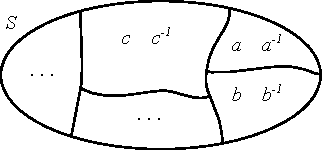
\includegraphics{img/chap4e.pdf}
   \end{figure}

   \noindent 1. In any finite group $G$, the number of elements not equal to 
   their own inverse is an even number.
   \begin{proof}
   The proof is trivial. The question is talking about the number of elements
   in $S$. The elements in $S$ can be paired off with their inverses. Therefore,
   there are $n$ pairs of elements. Therefore, there are $2n$ elements, which
   is always an even number.
   \end{proof}

   \noindent 2. The number of elements of $G$ equal to their own inverse is
   odd or even, depending on whether the number of elements in $G$ is odd
   or even.
   \begin{proof}
   Let the number of elements in $G$ be an even number, $2m$. From E1 we know
   that the number of elements not equal to their inverse is some even number, 
   $2n$. Therefore, the number of elements equal to their inverse is 
   $2m - 2n = 2(m-n)$ which is always even.

   Next consider that the number of elements in $G$ is some odd number
   $2m + 1$. Then the number of elements equal to their inverse is
   $(2m + 1) - 2n = 2(m-n) + 1$ which is always an odd number.
   \end{proof}

   \noindent 3. If the order of $G$ is even, there is at least one element
   $x$ in $G$ such that $x \ne e$ and $x = x^{-1}$.

   \begin{proof}
   The number of elements in $G$ is even. From E1 we know that the number of
   elements in $G$ that are equal to their own inverse is even. So we know
   that one of the elements that is equal to its own inverse is $e$. That gives
   us 1 element. Since the number of such elements is even, there must be at
   least one other $x$ in $G$ such that $x = x^{-1}$ and this element must not
   be equal to $e$ or we would still only have an odd number of such elements.
   \end{proof}

   \noindent In parts 4 to 6, let $G$ be a finite \emph{abelian} group, 
   say, $G = \{ \epsilon, a_1, a_2, \ldots , a_n\}$. Prove the following:

   \noindent 4. $(a_1a_2\cdots a_n)^2 = e$
   \begin{proof}
      We can expand $(a_1a_2 \cdots a_n)^2$ to $(a_1a_2\cdots a_na_1a_2 \cdots
      a_n)$. Then we can use commutative property to place each element next to
      it's inverse (either itself if it is equal to it's own inverse, or
      another elemtn that is its inverse). Now that every element is place next
      to it's inverse we can simplify the entire expression to $e$.
   \end{proof}

   \noindent 5. If there is no element $x \ne e$ in $G$ such that
   $x=x^{-1}$, then $a_1a_2 \cdots a_n = e$.
   \begin{proof}
   First observe that $G$ must have an odd number of elements. (If it
   had an even number of elements, then by E3 there must be an element
   $x \ne e$ such that $x=x^{-1}$. In that case the stated assumption
   does not hold.) We know that one of the elements is $e$. That leaves
   an even number of elements each of which must have an inverse in $G$.
   We can use the commutative property to place each element next to
   it's inverse, and then simplify to $e$.
   \end{proof}

   \noindent 6. If there is exactly one $x \ne e$ in $G$ such that
   $x=x^{-1}$, then $a_1a_2 \cdots a_n = x$.

   \begin{proof}
   Observe that there must be an even number of elements. There is
   $e$ and $x$ and then an even number of elements that are not 
   equal to their own inverse (by E1). By commuatitive property, we
   can align all the pairs next to each other and they all simplify to
   $e$. That leaves $x$.
   \end{proof}

   \item \textsc{Constructing Small Groups}

   \noindent In each of the following, let $G$ be any group. Let $e$ denote 
   the neutral element of $G$.

   \noindent 1. If $a,b$ are any elements of $G$, prove each of the 
   following:

   \begin{enumerate}[(a)]
      \item If $a^2 = a$, then $a=e$.
      \begin{proof}
      \begin{align*}
         a^2 & = a && \text{Given} \\
	 aa  & = a && \\
	 aaa^{-1} & = aa^{-1} \\
	 a   & = e \qedhere
      \end{align*}
      \end{proof}
      
      \item If $ab=a$, then $b=e$.
      \begin{proof}
         \begin{align*}
	    ab & = a   && \text{Given} \\
	    ab & = ae  && \text{Neutral element} \\
	    b & = e    && \text{Theorem 1} \qedhere
	 \end{align*}
      \end{proof}

      \item If $ab=b$, then $a=e$.
      \begin{proof}
         \begin{align*}
	    ab & = b   && \text{Given} \\
	    ab & = eb  && \text{Neutral element} \\
	    a  & = e   && \text{Theorem 1} \qedhere
	 \end{align*}
      \end{proof}

      \noindent 2. Explain why every row of a group table must contain each
      element of the group exactly once. (\textsc{Hint}: Suppose $x$
      appears twice in the row of $a$:

      \begin{table}[ht]
      \begin{tabular}{c|ccccc}
               & $\cdots$ & $y_1$    & $\cdots$ & $y_2$    & $\cdots$ \\ \hline
      $\vdots$ &          & $\vdots$ &          & $\vdots$ &          \\
             a & $\cdots$ & $x$      & $\cdots$ &  $x$     &          \\
      \end{tabular}
      \end{table}
      Now use the cancellation law for groups.)

      \begin{proof}
      As the hint suggests, let's assume that $x$ appears twice. Then we
      have $ay_1 = x = ay_2$. By the cancellation law for groups we
      have $y_1=y_2$ which contradicts are assumption that $y_1$ and
      $y_2$ where distinct elements in $G$. Therefore, every element
      of $G$ must show up in each row exactly once.
      \end{proof}

      \noindent 3. There is \emph{exactly one group} on any set of three
      distinct elements, say the set $\{e,a,b\}$. Indeed, keeping in mind
      parts 1 and 2 above, there is only one way of completing the following
      table. Do so! \emph{You need not prove associativity.}

      \begin{center}
      \begin{tabular}{c|ccc}
           & e & a & b \\ \hline
         e & e & a & b \\
	 a & a & b & e \\
	 b & b & e & a
      \end{tabular}
      \end{center}

      \tiny \begin{verbatim}

      \end{verbatim}
      \normalsize

      \noindent 4. There is exactly one group $G$ of four elements, say
      $G = \{e,a,b,c\}$, satisfying the additional property that
      $xx = e$ for every $x \in G$. Using only part 1 above, complete
      the following group table of $G$:

      \tiny \begin{verbatim}

      \end{verbatim} \normalsize
      \begin{center}
      \begin{tabular}{c|cccc}
           & e & a & b & c \\ \hline
	 e & e & a & b & c \\
	 a & a & e & c & b \\
	 b & b & c & e & a \\
	 c & c & b & a & e
      \end{tabular}
      \end{center}
      \tiny \begin{verbatim}

      \end{verbatim} \normalsize

      \noindent 5. There is exactly one group $G$ of four elements, say
      $G = \{e,a,b,c\}$, such that $xx=e$ for some $x\ne e$ in $G$, and
      $yy \ne e$ for some $y \in G$ (say, $aa=e$ and $bb\ne e$). Complete
      the group table of $G$, as in the preceding exercise.
      \tiny \begin{verbatim}

      \end{verbatim} \normalsize
      \begin{center}
      \begin{tabular}{c|cccc}
           & e & a & b & c \\ \hline
	 e & e & a & b & c \\
	 a & a & e & c & b \\
	 b & b & c & a & e \\
	 c & c & b & e & a
      \end{tabular}
      \end{center}
      \tiny \begin{verbatim}

      \end{verbatim} \normalsize

      \noindent 6. Use Exercise E3 to explain why the groups in parts 4
      and 5 are the only possible groups of four elements (except for
      renaming the elements with different symbols).

      \begin{proof}
      By inspection. Hard to explain. There are only 9 positions
      up for grabs. The constraints from part 3 constrain the choices.
      \end{proof}

      \item \textsc{Direct Products of Groups}

      \noindent If $G$ and $H$ are any two groups, their
      \emph{direct product} is a new group, denoted by $G \times H$,
      and defined as follows: $G \times H$ consists of all the ordered
      pairs $(x,y)$ where $x$ is in $G$ and $y$ is in $H$. That is,

      \[ 
         G \times H = \{(x,y) : x \in G \text{ and } y \in H \} 
      \] 

      The operation of $G \times H$ consists of multiplying corresponding
      components:

      \[ 
         (x,y)\cdot(x',y') = (xx',yy') 
      \]

      If $G$ and $H$ are denoted additively, it is customary to denote
      $G \times H$ additively:

      $$ (x,y)+(x',y') = (x+x',y+y') $$

      \noindent 1. Prove that $G \times H$ is a group by proving
      the three group axioms, ($G1$) to ($G3$):
      \begin{enumerate}[(G1)]
         \item \begin{align*}
	    (x_1,y_1)[(x_2,y_w)(x_3,y_3)] & = (x_1,y_1)(x_2x_3,y_2y_3) \\
	                                  & = (x_1x_2x_3,y_1y_2y_3) \\
	    [(x_1,y_1)(x_2,y_2)](x_3,y_3) & = (x_1x_2,y_1y_2)(x_3,y_3) \\
	                                  & = (x_1x_2x_3,y_1y_2y_3)
	 \end{align*}

	 \item Let $e_G$ be the identity element of $G$, and $e_H$
	 be the identity element of $H$. The identity element of
	 $G \times H$ is $(e_G,e_H)$:
	 \begin{align*}
	    (x,y)(e_G,e_H) & = (xe_G,ye_H)  \\
	                   & = (x,y)
	 \end{align*}

	 \item For each $(a,b)\in G \times H$, the inverse of $(a,b)$
	 is $(a^{-1},b^{-1})$:
	 \begin{align*}
	    (a,b)(a^{-1},b^{-1}) & = (aa^{-1},bb^{-1}) \\
	                         & = (e_G,e_H)
	 \end{align*}
      \end{enumerate}

      \noindent 2. List the elements of $\mathbb{Z}_2 \times \mathbb{Z}_3$,
      and write the operation table. (\textsc{Note}: There are six
      elements, each of which is an ordered pair. The notation is additive.)
      
      \Solution Remember that $\mathbb{Z}_2 = \{0,1\}$ and $\mathbb{Z}_3 =
      \{0,1,2\}$. This means $\mathbb{Z}_2 \times \mathbb{Z}_3 =
      \{(0,0), (0,1), (0,2), (1,0), (1,1), (1,2)\}$.

      \tiny \begin{verbatim}
      
      \end{verbatim}\normalsize
      \begin{center}
      \begin{tabular}{c|cccccc}
        +   & (0,0) & (0,1) & (0,2) & (1,0) & (1,1) & (1,2) \\ \hline
      (0,0) & (0,0) & (0,1) & (0,2) & (1,0) & (1,1) & (1,2) \\
      (0,1) & (0,1) & (0,2) & (0,0) & (1,1) & (1,2) & (1,0) \\
      (0,2) & (0,2) & (0,0) & (0,1) & (1,2) & (1,0) & (1,1) \\
      (1,0) & (1,0) & (1,1) & (1,2) & (0,0) & (0,1) & (0,2) \\
      (1,1) & (1,1) & (1,2) & (1,0) & (0,1) & (0,2) & (0,0) \\
      (1,2) & (1,2) & (1,0) & (1,1) & (0,2) & (0,0) & (0,1) 
      \end{tabular}
      \end{center}
      \tiny \begin{verbatim}
      
      \end{verbatim}\normalsize

      \noindent 3. If $G$ and $H$ are abelian, prove that $G \times H$
      is abelian.

      \begin{proof}
      \begin{align*}
         (x,y)(x',y') & = (xx',yy') \\
	 (x',y')(x,y) & = (x'x,y'y) \\
	              & = (xx',yy') && \text{Commutativity on $G$ and $H$}
		      \qedhere
      \end{align*}
      \end{proof}

      \noindent 4. Suppose the groups $G$ and $H$ both have the following
      property:
      \begin{figure}[ht]
          \emph{Every element of the group is its own inverse}
      \end{figure}

      Prove that $G\times H$ has this property.

      \begin{proof}
         \begin{align*}
	    (a,b)(a,b) & = (aa,bb)  \\
	               & = (aa^{-1},bb^{-1}) && \text{Given} \\
		       & = (e_G,e_H) \qedhere
	 \end{align*}
      \end{proof}

   \end{enumerate}
\end{enumerate}




\end{document}
